\documentclass{article}
\usepackage{amsmath}
\usepackage{amssymb}
\usepackage{amstext}
\usepackage{bussproofs}
\usepackage{tikz}

\title{HoTTEST Summer School 2022 \\
  Lecture 1 \\
  Dependent Type Theory and $\Pi$-Types}
\author{ Lecture by Paige North \\
Notes by Peter Fortin}
\date{July 4 2022}


\begin{document}

\maketitle
\tableofcontents

\section{Homotopy Type Theory}

Homotopy type theory brings out connections between three different
aspects of mathematics: foundations, formalization, and practice. 
There are deep connections between all of these fields, and HoTT
gives a framework to view all of these connections from a central
perspective. Fields such as type theory and functional programming
give computational interpretations to HoTT. The connections between 
logic, set theory, and topos theory allow us to view HoTT as a 
foundation for all of mathematics. And finally, homotopy theory,
category theory, topos theory, and other areas of abstract mathematics
give us useful fields to use the tools and techniques that HoTT provides
in order to do actual mathematics.

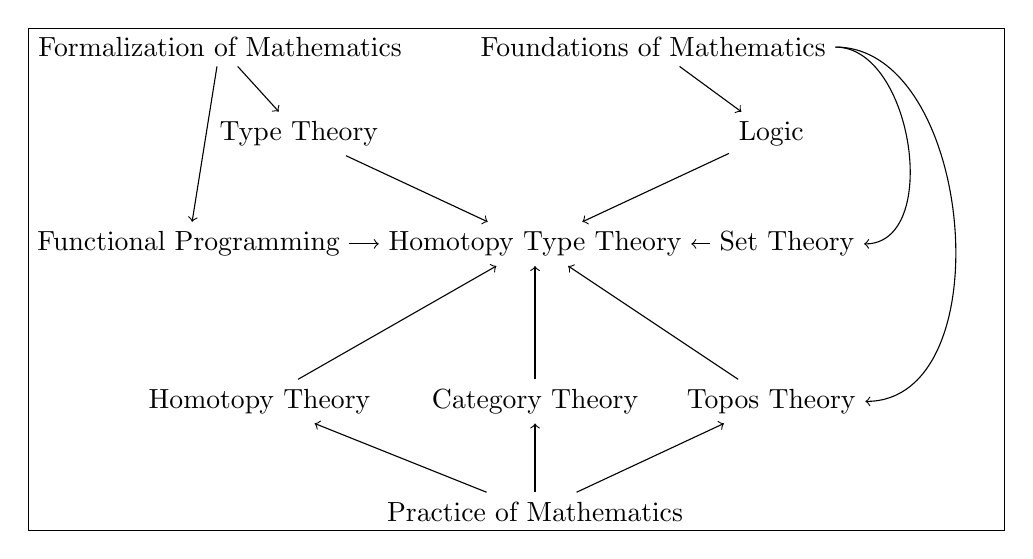
\begin{tikzpicture}
    
    \coordinate (C1)  at (-4, 2.5);
    \coordinate (C2)  at (1.5, 2.5);
    \coordinate (C3)  at (-3, 1.4);
    \coordinate (C4)  at (3, 1.4);
    \coordinate (C5)  at (-4.4, 0);
    \coordinate (C6)  at (0, 0);
    \coordinate (C7)  at (3.2,0);
    \coordinate (C8)  at (-3.5, -2);
    \coordinate (C9)  at (0, -2);
    \coordinate (C10) at (3, -2);
    \coordinate (C11) at (0, -3.4);

    

    \node (N1)  at (C1)  {Formalization of Mathematics};
    \node (N2)  at (C2)  {Foundations of Mathematics};
    \node (N3)  at (C3)  {Type Theory};
    \node (N4)  at (C4)  {Logic};
    \node (N5)  at (C5)  {Functional Programming};
    \node (N6)  at (C6)  {Homotopy Type Theory};
    \node (N7)  at (C7)  {Set Theory};
    \node (N8)  at (C8)  {Homotopy Theory};
    \node (N9)  at (C9)  {Category Theory};
    \node (N10) at (C10) {Topos Theory};
    \node (N11) at (C11) {Practice of Mathematics};

    \draw [->] (N1) -- (N3);
    \draw [->] (N1) -- (N5);

    \draw [->] (N2) -- (N4);
    \draw [->] (N2) to [out=0,in=0] (N7);
    \draw [->] (N2) to [out=0,in=0] (N10);

    \draw [->] (N11) -- (N10);
    \draw [->] (N11) -- (N9);
    \draw [->] (N11) -- (N8);

    \draw [->] (N3)  -- (N6);
    \draw [->] (N4)  -- (N6);
    \draw [->] (N5)  -- (N6);
    \draw [->] (N7)  -- (N6);
    \draw [->] (N8)  -- (N6);
    \draw [->] (N9)  -- (N6);
    \draw [->] (N10) -- (N6);

    \draw (current bounding box.north east) rectangle (current bounding box.south west);

\end{tikzpicture}

\begin{center}
    A Map of the Territory
\end{center}

\section{Logic and Natural Deduction}

Natural Deduction is a proof system for logic which uses rules 
of inference to create proofs of propositions. When referring to the formal system,
we will call it \textbf{ND}. Propositions are
declarative statements which can be either true or false.
Proofs in \textbf{ND} are trees where each branch is the application and result 
of some rule. 

Rules in \textbf{ND} always come in pairs: introduction and elimination.
Each logical notion has a way of introducing it and a way of eliminating it.
These rules require some sort of hypothesis. We represent this
by writing what is assumed to be true above a vertical bar, and the 
conclusion, or what comes after the use of the rule, on the bottom of the bar. 
A proof is then a tree where the root is the conclusion and all of the 
premises are the end leaves.

We have two rules, $\times$ and $\rightarrow$. $P \times Q$ is conjunction, 
which means we are taking the propositions $P$ and $Q$ to both be true at the
same time. $P \rightarrow Q$ is implication, which means we take the truth
of $P$ to imply the truth of $Q$.


\begin{prooftree}
  \AxiomC{$P$}
  \AxiomC{$Q$}
     \RightLabel{$\times$-intro}
  \BinaryInfC{ $P \times Q$}
\end{prooftree}

\begin{center}
    \AxiomC{$P \times Q$}
  \RightLabel{$\times$-elim-l}
    \UnaryInfC{ $P$ }
  \DisplayProof
  \hspace{1cm}
    \AxiomC{$P \times Q$}
  \RightLabel{$\times$-elim-r}
    \UnaryInfC{$Q$}
  \DisplayProof

\end{center}

\begin{center}
    \textbf{ND} rules for $\times$
\end{center}

The $\times$-intro rule means that if we have proven $P$ and we have proven
$Q$, we can infer$ P \times Q$. $\times$-elim-l means that if we have we have
proven $P \times Q$, we can infer $P$ alone, and $\times$-elim-r means the same,
but for $Q$. The intuition is that once we have proven a conjunction, we can get
either of the conjuncts by themselves, which is the inverse of how we prove
the conjunction in the first place.


\begin{center}

    \AxiomC{[$P$]}
    \noLine
    \UnaryInfC{.}
    \noLine
    \UnaryInfC{.}
    \noLine
    \UnaryInfC{.}
    \noLine
    \UnaryInfC{$Q$}
    \RightLabel{$\rightarrow$-intro}
    \UnaryInfC{$P \rightarrow Q$}
    \DisplayProof
    \hspace{1cm}
    \AxiomC{$P$}
    \AxiomC{$P \rightarrow Q$}
    \RightLabel{$\rightarrow$-elim}
    \BinaryInfC{$Q$}
    \DisplayProof

\end{center}

\begin{center}
    \textbf{ND} rules for $\rightarrow$
\end{center}

The $\rightarrow$-intro rule means that under the assumption that $P$ is true,
if we then go on to legally infer $Q$, we can infer that $P \rightarrow Q$. It
is important to understand that we can assume $P$ to be true for the purposes
of inferring an $\rightarrow$-intro even if we don't know that $P$ is true. 
This is because we are not trying to prove $P$, we are trying to prove
$P \rightarrow Q$. The $\rightarrow$-elim rule, which is called modus ponens,
means that if we have proven $P$, and if we have proven that $P \rightarrow Q$,
then we can put those two together to derive $Q$. 

Introduction rules tell us how to produce a proof of some statement. elimination
rules tell us what we can do with that statement (which, usually, is prove more
statements).

It should be noted that if we think of types as sets and terms as elements,
then conjunction and all of these rules behave exactly like the set theoretic
Cartesian product. Additionally, conjunction has a lot of rules simply because
it involves a left and a right side.

\section{The Simply Typed Lambda Calculus}

The Simply Typed Lambda Calculus (\textbf{ST$\Lambda$C}) is a model of 
computation, and is closely related to \textbf{ND}. \textbf{ST$\Lambda$C}
is what we get when we make \textbf{ND} \emph{proof relevant}. This means
that we don't only care about the abstract idea that some proposition is true.
Instead, we carry around explicit proofs of the truth along with the proposition.

In \textbf{ND} we write ``$P$" to mean``$P$ holds", but in \textbf{ST$\Lambda$C} we 
write ``$p : P$" to mean ``$p$ is a proof/witness of $P$". We say $p$ is a \emph{term} 
of \emph{type} $P$. Because types are their own concept in \textbf{ST$\Lambda$C},
we also have rules for determining that something has a specific type, and
we call these ``formation" rules, and they exist along with the corresponding
introduction and elimination rules. Finally, because \textbf{ST$\Lambda$C} is
a model of computation, we need computation rules to tell us how to compute
with our terms and types. Computation rules often come in pairs as well,
$\beta$ and $\eta$ rules. Below are the \textbf{ST$\Lambda$C} rules for $\times$:

\pagebreak

\begin{center}
    \AxiomC{$P$ Type}
    \AxiomC{$Q$ Type}
    \RightLabel{$\times$-form}
    \BinaryInfC{$P \times Q$ Type}
    \DisplayProof
\end{center}

\begin{center}
    \AxiomC{$\Gamma \vdash p : P$}
    \AxiomC{$\Gamma \vdash q : Q$}
    \RightLabel{$\times$-intro}
    \BinaryInfC{$\Gamma \vdash (p, q) : P \times Q$}
    \DisplayProof
\end{center}

\begin{center}
    \AxiomC{$\Gamma \vdash a : P \times Q$}
    \RightLabel{$\times$-elim-l}
    \UnaryInfC{$\Gamma \vdash \pi_1 a : P$}
    \DisplayProof
    \hspace{1cm}
    \AxiomC{$\Gamma \vdash a : P \times Q$}
    \RightLabel{$\times$-elim-r}
    \UnaryInfC{$\Gamma \vdash \pi_2 : Q$}
    \DisplayProof
\end{center}

\begin{center}
    \AxiomC{$\Gamma \vdash p : P$}
    \AxiomC{$\Gamma \vdash q : Q$}
    \RightLabel{$\times$-comp-$\beta$-l}
    \BinaryInfC{$\Gamma \vdash \pi_1(p,q) \doteq p : P$}
    \DisplayProof
\end{center}

\begin{center}
    \AxiomC{$\Gamma \vdash p : P$}
    \AxiomC{$\Gamma \vdash q : Q$}
    \RightLabel{$\times$-comp-$\beta$-r}
    \BinaryInfC{$\Gamma \vdash \pi_2(p,q) \doteq q : Q$}
    \DisplayProof
\end{center}

\begin{center}
    \AxiomC{$\Gamma \vdash a : P \times Q$}
    \RightLabel{$\times$-comp-$\eta$}
    \UnaryInfC{$\Gamma \vdash (\pi_1 a, \pi_2 a) \doteq a : P \times Q$}
    \DisplayProof
\end{center}

\begin{center}
    \textbf{ST$\Lambda$C} rules for $\times$
\end{center}

There are a few new symbols here. $\Gamma$ is called a \emph{context}. 
It is a variable which stands for a collection of hypotheses, which could be empty. 
The idea is that we don't want our rules to only apply when we have nothing but the 
terms involved in the proof; we want to be able to use our rules at any point during a 
proof. So $\Gamma$ stands for whatever has been proven before, which could be nothing 
at all, e.g. if we're at the first step of our proof. 

$\vdash$ is a meta way of expressing implication, similar to how we use the underline
bar. When we write something like $\Gamma \vdash \Delta$, we are saying that the
context $\Gamma$ proves the context $\Delta$. Often times, we will make some of
the terms in either of the two contexts explicit, since they are the terms we want
to manipulate. These ``metavariables'' exist to show that we are accounting for all
of the proofs which have already been derived, even if that is an empty set. The 
$\times$-form rule tells us that, much like in \textbf{ND}, if we have that $P$ is
a type and $Q$ is a type, then $P \times Q$ is a type. 

$\pi_1$ and $\pi_2$ are projections. They represent the idea of taking the conjunction
$a : P \times Q$ and ``extracting'' the $P$ and the $Q$ parts, respectively. The 
elimination rules tell us how we can turn an $a : P \times Q$ into its respective
projections, that is, the parts of it which have types $P$ and $Q$. The combination
of the introduction and elimination rules tells us that if we have two types $P$ 
and $Q$, we can always put them together and take them apart again.

The computation rules introduce the idea of \emph{judgmental equality}. Our
type rules, as well as any time we express that a term is of a type, e.g. $p : P$,
we are making a \emph{judgement} in our theory. The expression 
$\Gamma \vdash p \doteq q : P$ is expressing the judgement that $p$
and $q$ are judgmentally equal terms of the type $P$. Again, much more
will be said about this later. As for the computation rules,
$\times$-comp$\beta$-l says that if $(p,q) : P \times Q$, then
the left projection $\pi_1 (p,q) : P$ is judgmentally equal to $p : P$ itself.
$\times$-comp$\beta$-r says the same but for the right projection. Finally,
$\times$-comp-$\eta$ says that if $a : P \times Q$, then it is judgmentally 
equivalent to the composition of its left and right projections. These computational
rules tell us how we can move between conjunctions and their constituent parts, and
that this process is guided by their types. Below are the \textbf{ST$\Lambda$C} 
rules for $\rightarrow$:

\begin{center}
    \AxiomC{$P$ Type}
    \AxiomC{$Q$ Type}
    \RightLabel{$\rightarrow$-form}
    \BinaryInfC{$P \rightarrow Q$ Type}
    \DisplayProof
\end{center}

\begin{center}
    \AxiomC{$\Gamma, x : P \vdash q : Q$}
    \RightLabel{$\rightarrow$-intro}
    \UnaryInfC{$\Gamma \vdash \lambda x . q : P \rightarrow Q$}
    \DisplayProof
    \hspace{1cm}
    \AxiomC{$\Gamma \vdash p : P$}
    \AxiomC{$\Gamma \vdash f : P \rightarrow Q$}
    \RightLabel{$\rightarrow$-elim}
    \BinaryInfC{$\Gamma \vdash f p : Q$}
    \DisplayProof
\end{center}

\begin{center}
    \AxiomC{$\Gamma , x : P \vdash q : Q$}
    \AxiomC{$\Gamma \vdash p : P$}
    \RightLabel{$\rightarrow$-comp-$\beta$}
    \BinaryInfC{$\Gamma \vdash (\lambda x . q) p \doteq q[p/x] : Q$}
    \DisplayProof
\end{center}

\begin{center}
    \AxiomC{$\Gamma \vdash f : P \rightarrow Q$}
    \RightLabel{$\rightarrow$-comp-$\eta$}
    \UnaryInfC{$\Gamma \vdash \lambda x . f x \doteq f : P \rightarrow Q$}
    \DisplayProof
\end{center}

\begin{center}
    \textbf{ST$\Lambda$C} rules for $\rightarrow$
\end{center}

The meaning of the formation rule should by now be obvious. The
$\rightarrow$-intro rule introduces a new symbol $\lambda$, which is
called lambda abstraction, and it also has an example of more than just
$\Gamma$ on the left hand side of a $\vdash$. What $\rightarrow$-intro
says is that if the context $\Gamma$, \emph{as well as} the context
of $x : P$ proves $p : Q$, then we can \emph{abstract} the term
$x : P$ over the term $q : Q$ as a witness to the fact that a term
of type $P$ can be used to prove $q : Q$. The computational interpretation
of this makes the situation much clearer. Similarly, $\rightarrow$-elim
says that we can supply a witness $p : P$ to a witness $f : P \rightarrow Q$
to get a witness $f p : Q$.

The computational interpretation of these rules comes from
$\rightarrow$-comp-$\beta$ and $\rightarrow$-comp-$\eta$. 
$\rightarrow$-comp-$\beta$ introduces another new symbol, $q[p/x] : Q$,
which is called substitution. The idea is to take $q : Q$ as a syntactic object,
which may or may not contain the syntactic object $x : P$, and then replace
each occurrence of $x : P$ with $p : P$. $\rightarrow$-comp-$\beta$ says that
the $\lambda$-abstraction \emph{applied to a term of the correct type}, is 
judgmentally equivalent to the term after the substitution takes place.
$\rightarrow$-comp-$\eta$ says that an implication is judgmentally equivalent to a 
$\lambda$-abstraction which takes a term of the right type and then applies the
implication.

As was stated above, \textbf{ST$\Lambda$C} is a model of computation.
These last two rules can be understood in a straightforwardly computational way.
Imagine that $f : P \rightarrow Q$ is a function. $\rightarrow$-comp-$\beta$
says that applying $f$ to an argument of the right type will produce a result
of the right type, and moreover, that the way the result is calculated is by
substituting the free variable bound by the $\lambda$-abstraction.
$\rightarrow$-comp-$\eta$ says that a function $\lambda x . f x$ which 
takes an argument and applies $f$ to that argument, is equivalent to $f$ itself.

The one-to-one connection between \textbf{ND} and \textbf{ST$\Lambda$C} is known as
the ``Curry-Howard Correspondence'', or ``Propositions as Types'', since it was
discovered by Haskell Curry and William Howard. The correspondence, as the second
name suggests, tells us that logic and computation are two sides of the same coin,
and that propositions operate in the exact same way as types. Proofs of propositions
correspond to programs which return the appropriate type. Under this correspondence,
the logical view of $\rightarrow$ is as implication, and the computational view is
as a function. This lets us use types as a means of program specification. We 
can turn a logical statement such as $P \rightarrow P$ into the specification
of a program $(\lambda x. x) : P \rightarrow P$ which takes an argument of type $P$
and produces a result of type $P$. Clearly, the only thing that this function
can do is to return what it was given. So the logical idea of a proposition
implying itself gives a specification for a program that returns its
input. The term of the type being specified is the program witnessing it's
proof.

Finally, we can now give a good explanation for notation like $\pi_1 a$. When
we have a term with a function/implication type $P \rightarrow Q$ and we set
it next to a term with type $P$, that should be taken to mean function 
application/modus ponens.


\section{Dependent Type Theory}

In \textbf{ND}, our deductions had no terms. That is, there was nothing
"inside" of the propositon variables $P$ and $Q$. The \textbf{ST$\Lambda$C} allowed
us to interpret $P$ as a type, and consequentally a judgement such as $p : P$ as 
asserting that the term $p$ has type $P$. Our judgemnts in \textbf{ST$\Lambda$C}
only allow us to make terms which depend on other terms. For example, 
$\rightarrow$-comp-$\beta$ tells us that we can form terms such as 
$(\lambda x. x) : P \rightarrow P$ under the condition that $x : P$. However,
the rules of \textbf{ST$\Lambda$C} \emph{only} allow us to have terms depend
on terms. 

Dependent type theory allows us to also have \emph{types} depend
on terms, and as such it is an extension of the \textbf{ST$\Lambda$C}. Under
the interpretation of types as propositions, dependent types are predicates. Under
the interpretation of types as sets, dependent types are indexed families of sets.
Under the interpretation of types as program types, dependent types are program type
specifications which involve a parameter.

We carry over the same rules as in the \textbf{ST$\Lambda$C}, except now
our type judgements also contain contexts,

\begin{center}
    \AxiomC{$\Gamma \vdash P$ Type}
    \AxiomC{$\Gamma \vdash Q$ Type}
    \RightLabel{$\rightarrow$-form}
    \BinaryInfC{$\Gamma \vdash P \rightarrow Q$ Type}
    \DisplayProof
\end{center}

\begin{center}
    \AxiomC{$\Gamma \vdash P$ Type}
    \AxiomC{$\Gamma \vdash Q$ Type}
    \RightLabel{$\times$-form}
    \BinaryInfC{$\Gamma \vdash P \times Q$ Type}
    \DisplayProof
\end{center}

The main concept dependent type theory adds to \textbf{ST$\Lambda$C} is
the idea of a dependent function type, $\prod$.

\section{Dependent Functions}

As an example of a dependent function, imagine that we have a 
type of natural numbers $\mathbb{N}$, and a type $Vect$ of all 
finite vectors consisting of natural numbers. We could define a function
$0 : \mathbb{N} \rightarrow Vect$ which takes a natural number $n$ as input 
and returns the vector of length $n$ whose components are all $0$.
But since we know that the output vector will always be of a certain length,
we also know that the vector isn't just an object in $Vect$, it's also an
object in $Vect(n)$, that is, the type of vectors of length $n$. Dependent
functions let us encode this special property of the function by specifiying how
the output type of the function \emph{depends} on the input term.

We have two ways of writing this, one is a ``type theory'' way, and one is
a computer science way. 

\begin{center}
    $0 : \prod_{n : \mathbb{N}} Vect(n)$
    \hspace{1cm}
    $0 : (n : \mathbb{N}) \rightarrow Vect(n)$
\end{center}

The logical interpretation of $\prod$ is as $\forall$, that is, it can 
be read as a universal quantifier. Dependent function types are generalizations
of regular function types, because in a regular function type, the result type does
not depend on a term from the input type. This is a special case of a dependently 
typed function where the return type does not depend on the input term, such as 
$0 : \prod_{n : \mathbb{N}} Vect$. The product type is also a special case of 
the dependent function type, but the proof requires more than what we have so 
far. This is important, however, because it shows the parsimony of definition in 
type theory. We normally don't define at the basic level individual types such as 
$\rightarrow$ or $\times$, since we can define them with $\prod$. Of course, though,
we needed to define them for \textbf{ND} and \textbf{ST$\Lambda$C}, because 
$\prod$ does not exist in those languages. We conclude with the rules for 
$\prod$ types.

\begin{center}
    \AxiomC{$\Gamma , x : P \vdash Q$ type}
    \RightLabel{$\prod$-form}
    \UnaryInfC{$\Gamma \vdash \prod_{x : P} Q$ type}
    \DisplayProof
    \hspace{0.5cm}
    \AxiomC{$\Gamma , x : P \vdash q : Q$}
    \RightLabel{$\prod$-intro}
    \UnaryInfC{$\Gamma \vdash \lambda x . q : \prod_{x : P} Q$}
    \DisplayProof
\end{center}

\begin{center}
    \AxiomC{$\Gamma \vdash f : \prod_{x : P} Q$}
    \AxiomC{$\Gamma \vdash p : P$}
    \RightLabel{$\prod$-elim}
    \BinaryInfC{$\Gamma \vdash fp : Q[p/x]$}
    \DisplayProof
\end{center}

\begin{center}
    \AxiomC{$\Gamma , x : P \vdash q : Q$}
    \AxiomC{$\Gamma \vdash p : P$}
    \RightLabel{$\prod$-comp-$\beta$}
    \BinaryInfC{$\Gamma \vdash (\lambda x . q)p \doteq q[p/x] : Q[p/x]$}
    \DisplayProof
\end{center}

\begin{center}
    \AxiomC{$\Gamma \vdash f : \prod_{x : P} Q$}
    \RightLabel{$\prod$-comp-$\eta$}
    \UnaryInfC{$\Gamma \vdash \lambda x . f x \doteq f : \prod{x : P}Q$}
    \DisplayProof
\end{center}


\begin{center}
    Dependent Type Theory rules for $\prod$
\end{center}

\end{document}

